\chapter{Organisation Effectiveness}

\section{Introduction}
In this section, we will analyse two companies using the \emph{7S framework}~\citep{waterman1980structure}.
This framework can be used to analyse the effectiveness of an organisation.
We will use the analysis to learn about the influence of RUP and Scrum on organisation effectiveness, and we will try to gain insight into what could have been done differently in the organisation of the failed case from the previous assignment.

\section{McKinsey 7S Framework}
The 7S framework~\citep{waterman1980structure} was proposed in 1980 by Robert H. Waterman, Jr. and Tom Peters, two business consultants who were working for the American business consultancy firm McKinsey at the time. During that period, there were concerns regarding organisation effectiveness among McKinsey's clients. The way in which an organisation was perceived was focused on structure and strategy alone; however, the consensus was that this way of looking at things is unsatisfactory and incomplete.

In response to this, the two developed a new framework for assessing and monitoring changes in the internal situation of an organisation. One which not only included structure and strategy as organisational factors but also five other factors in order to help diagnose causes of organisational problems. The model is based on the theory that, for an organisation to perform well, these seven elements need to be aligned and mutually reinforcing. A graphical depiction of the framework is presented in figure~\ref{fig:sevens_framework}.

\begin{figure}[!ht]
    \centering
        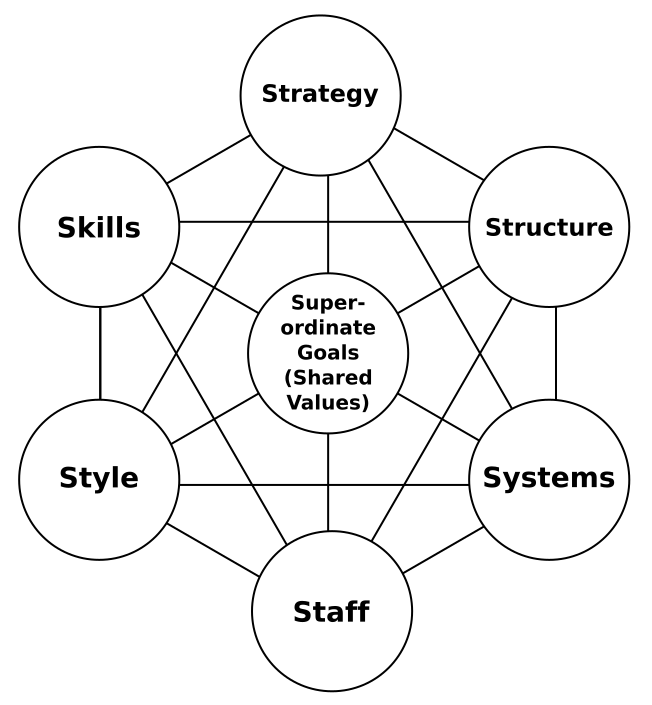
\includegraphics[width=0.6\textwidth]{graphics/sevens_framework}
    \caption{The 7S framework}
    \label{fig:sevens_framework}
\end{figure}

The model emphasises the interdependence of the factors using the connections between them. One factor may influence others, and all of them must be aligned in order for an organisation to be well organised. Also, the model is deliberately shaped in a way that does not communicate hierarchy because one factor is not necessarily more important than the others.

A brief explanation of the seven factors in terms of what question(s) each factor tries to answer:
\begin{description}
    \item[Strategy] What does the organisation do to provide added value?
    \item[Skills] What are the competencies both at the organisation level and at the level of its people?
    \item[Structure] How is the organisation arranged?
    \item[Style] How do leaders operate and interact within the organisation?
    \item[Systems] What are the rules, regulations, and processes with regard to getting things done and management activities?
    \item[Staff] How does the organisation make sure it has the right people?
    \item[Shared Values] What are the core beliefs in the organisation about what is important and why the organisation exists?
\end{description}

\section{IKEA}
- required non-software company
- largest furniture retailer of the world since 2008
- known for self-assembly furniture
- interesting because world-leading company

\paragraph{Strategy}
\citep{kumar2000market}
- design: in-house as opposed to independent
- design: simple as opposed to complex
- parts: modular-interchangeable parts as opposed to high level-wip
- parts: cheap, mass production as opposed to expensive hand-made
- assembly: self-assembly as opposed to built-to-order
- transport: efficient and computerised due to mass produced modular parts as opposed to (inefficient) transport of costly, bulky finished product
- marketing: leverage Scandinavian image and cheap out-of-town display as opposed to fragmented image across geographies and expensive high-street display
- service: self-service and self-transport vs full-service and delivery

\paragraph{Systems}

\paragraph{Structure}

\paragraph{Skills}

\paragraph{Shared values}

\paragraph{Staff}

\paragraph{Style}


% START OF GOOGLE SECtiON
\section{Google}

\paragraph{Strategy}
Google's public vision is not stated clearly on their website. Other sources indicate that the following is Google's vision: ``to provide access to the world’s information in one click''\footnote{\url{http://panmore.com/google-vision-statement-mission-statement}}. Nowadays, Google is known for many services. However, one service is at the core of Google: search. Needless to say that there are still many challenges in that area. Nonetheless, Google is dedicated to keep investing in this area and explore new techniques and methods to change the status quo.

\paragraph{Systems}
In general, Google teams tend to use agile methods. Some teams adopt XP or Scrum, but there is no company guideline as to which methodology to use. Most teams are self-organising and are free to choose whatever software processes they see fit. Teams often do not even have a project manager assigned; teams communicate directly with stakeholders \citep{striebeck2006ssh}. Google's management does not want to impose methodologies on teams and overburden them. Management believes that the teams themselves know what processes would work best for them. The software process is intentionally not centralised, and a person working at Google even claims that Google's philosophy is the exact opposite of something like CMMI\footnote{\url{https://www.quora.com/What-software-development-methodology-ies-does-Google-use}} that requires certain processes to be put in place. If one team discovers that a certain practise works well for them, other teams will follow \citep{striebeck2006ssh}. Thus, there is a lot of experimentation going on at any point in time.

The AdWords team is the exception to this philosophy, in that more standards are imposed on the process employed. This is because AdWords is much more business input driven than other projects. The AdWords project does have project managers and a fairly large management team. Some projects tried to use Agile practises, but not every practice was introduced at the same time. Team members needed to become accustomed and see the benefit of a certain practice before others are introduced. Post-mortems are conducted at the end of a project, and positive and negative points of certain methodologies are reviewed in order to decide which practises should be employed in future projects. Certain practises can be modified or improved based on this feedback. Slowly, some teams that were initially reluctant to adopt formal software processes saw the value of using certain Agile practises.

Peer reviewing is required for all code written\footnote{\url{http://steve-yegge.blogspot.nl/2006/09/good-agile-bad-agile_27.html}}. When it comes to writing code, engineers are very disciplined. The result is that the whole codebase looks the same, so it's easier for people to switch teams.

\paragraph{Structure}
The organisational structure of Google can be classified as a matrix organisation, although it is one with a rather flat hierarchy. Teams are assigned by function and by product. For example, a web developer is assigned to the Engineering \& Design\footnote{\url{https://www.google.com/about/careers/teams/}} team, as well as the Google+ team. Google's organisational structure is relatively flat. That is, there hardly is any middle management and the upper management can be approached quite easily.

\paragraph{Skills}
In the past, Google, as a company, excelled in quick decision making. When Larry Page took over as CEO in 2012 and reformed decision making at the company\footnote{\url{https://www.thinkwithgoogle.com/articles/start-up-speed-kristen-gil.html}}, he believed that as the company had grown, it had become less agile\footnote{\url{http://michael-roberto.blogspot.nl/2012/01/larry-page-reforms-decision-making-at.html}}. Another area of competence is the ability to provide more relevant search results than its competitors, particularly because of the development of the PageRank algorithm.

\paragraph{Shared values}
As of 2016, Google has the following mission: "to organise the world’s information and make it universally accessible and useful."\footnote{\url{https://www.google.com/intl/en/about/}}. Google encourages risk taking, non-traditional thinking, and innovation by employees\footnote{\url{http://2012books.lardbucket.org/books/an-introduction-to-organizational-behavior-v1.1/s15-01-decision-making-culture-the-ca.html}}. In addition, Google deeply values integrity, collaboration, and trust \citep{striebeck2006ssh}. The following quote conveys those shared values: "When a vice president in charge of the company’s advertising system made a mistake costing the company millions of dollars and apologised for the mistake, she was commended by Larry Page, who congratulated her for making the mistake and noting that he would rather run a company where they are moving quickly and doing too much, as opposed to being too cautious and doing too little."\footnote{\url{https://www.linkedin.com/pulse/20140904061228-154884582-organizational-culture-in-google-inc}}. Thus, making mistakes is accepted, and agility is a shared value. This has consequences for the software processes in place at the company. After all, a new process, such as Scrum, may be experimented with on a small scale to see if it works out and the rest of the company should adopt it. This is also why Google allows employees to spend 20\% of their time on their own ideas.
Founder Sergey Brin states that the company's culture should not be static; it should continuously improve. This may facilitate adoption of new software processes. Google has even appointed a 'chief culture officer' to guide this.

\paragraph{Staff}
Google's hiring policy is that they only recruit the brightest and best individuals. In terms of Etzioni's compliance theory\citep{lunenburg2013compliance}, Google can be classified as being a Normative-Moral organisation when considering the type of power they use to direct the behaviour of their members and the type of involvement of the participants. Normative because most employees share the vision to innovate and passion for the company to succeed and change the state of technology. Moral because employees are proud to work at Google and are often loyal to the company, staying with the company for years at end.

\paragraph{Style}
It is publicly known that Google values decisions made by teams\footnote{\url{https://www.linkedin.com/pulse/20140904061228-154884582-organizational-culture-in-google-inc}}, as opposed to decision making by single individuals. Until recently, high-level decisions were made consensually by founders Larry Page and Sergey Brin, accompanied by CEO Eric Schmidt. Google does not enforce decision making in a top-down way. Rather, it stresses the importance of rational persuasion, and teams may propagate these decisions bottom-up. Amit Singh (Google's senior vice-president and head for worldwide enterprise services) states: "We believe in bottoms-up decision making"\footnote{\url{http://articles.economictimes.indiatimes.com/2013-12-24/news/45540233_1_chrome-os-chromebooks-hangouts}}. It is also believed that top-down decision making leads to organisational anarchy. The emphasis here is on rational, thus every decision should involve proper argumentation and should not be based on instinct or feeling.

Employees at Google usually work in open office environments. The reason behind this is the conviction that open offices foster teamwork.

% END OF GOOGLE SECTION

\section{Lessons learned}
From Google's approach we can learn that in some cases it works great to give autonomy to teams. But active experimentation is valuable too, because only then will people notice if something makes a difference or not. It also shows us that a bottom-up approach works in the case of a technological company.

\subsection{RUP}

\subsection{SCRUM}

\subsection{Failed Case}

\section{Conclusion}